% 图 78.4 —— 由 `checks/emit_hand.py` 自动拼出（probe 精测 + prims2 图元分解）
%%
% ⚠ 这是**稿子不是成品**：跑 `checks/checkhand.py 78.4` 看指标 + 看叠合图。
%%
%% ⚠ 待核：
%   · 本图 probe 报出阴影族 1 个 —— **本脚本不生成阴影**（要照原书手写）；prims2 的 strokes 里可能含阴影线，核对时留意别画重
%   · 可疑字形 2 项（空心圈 ⊙ 常被认成字母 o）—— 见文件末
%%
\documentclass[12pt]{standalone}
\usepackage{fontspec}
\setsansfont{Arial}
\newfontfamily\mfallback{DejaVu Sans}
\usepackage{tikz}
\begin{document}
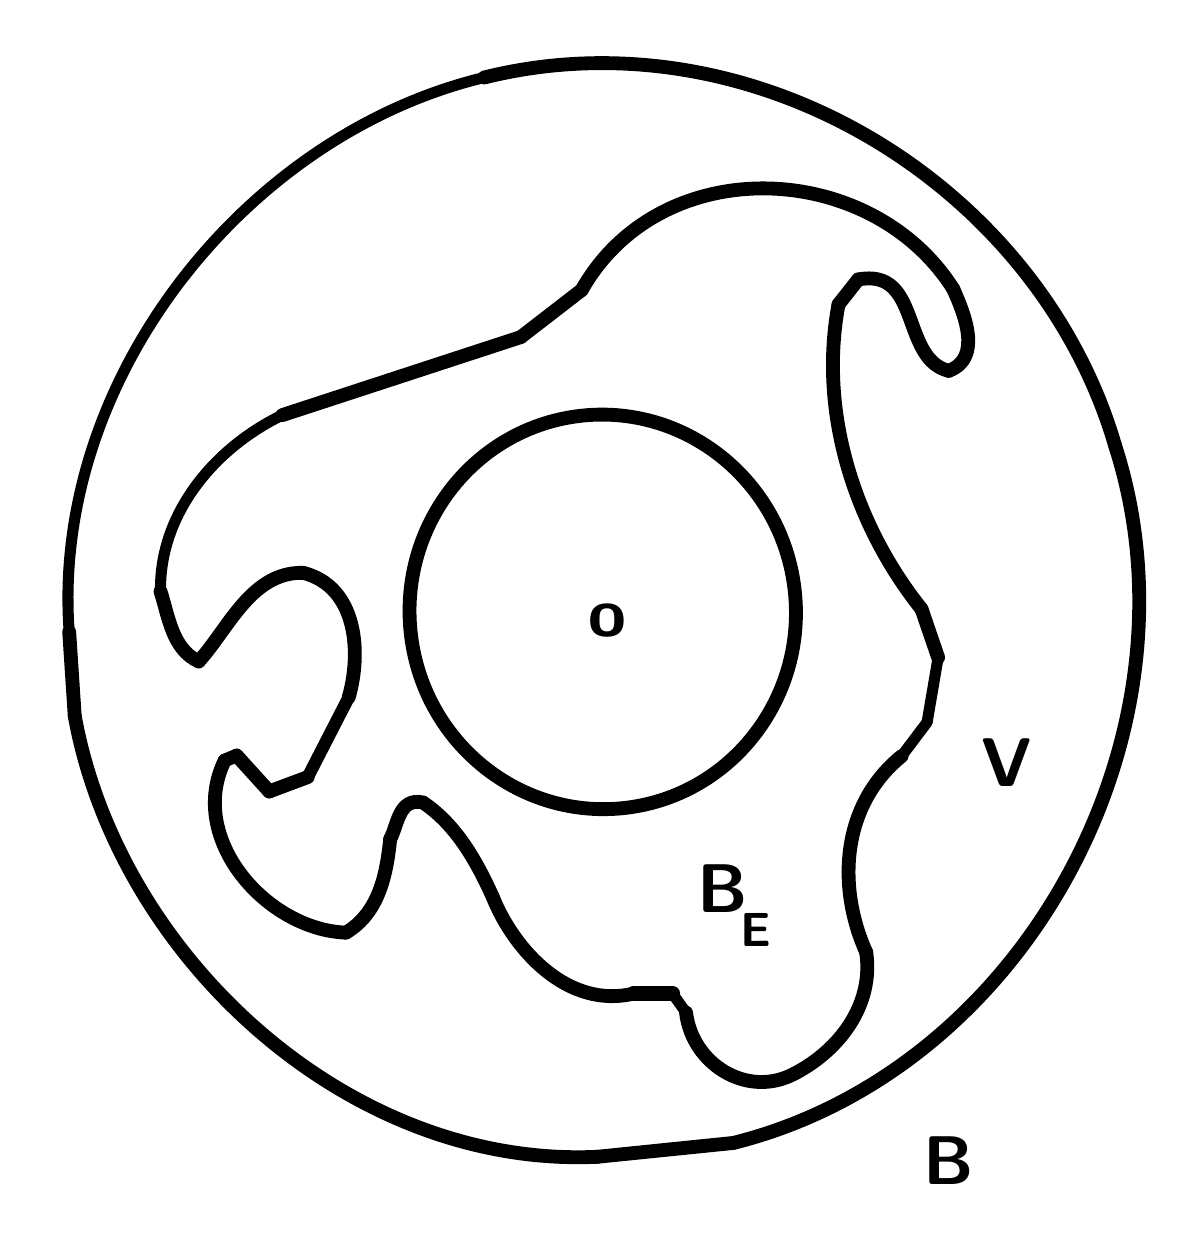
\begin{tikzpicture}[x=1pt, y=-1pt, line width=5.0pt, line cap=round, line join=round]

  %% ════ 直线段（prims2 的 strokes）════
  \draw[line width=5.0pt] (15.0,218.3) -- (17.0,248.7);
  \draw[line width=5.0pt] (205.9,408.0) -- (255.0,403.0);
  \draw[line width=4.9pt] (71.2,264.8) -- (75.5,263.0);
  \draw[line width=5.0pt] (75.5,263.0) -- (87.3,276.0);
  \draw[line width=5.0pt] (87.3,276.0) -- (101.2,270.8);
  \draw[line width=4.5pt] (101.2,270.8) -- (116.0,242.0);
  \draw[line width=5.0pt] (92.0,140.0) -- (178.2,111.8);
  \draw[line width=5.0pt] (178.2,111.8) -- (200.2,94.8);
  \draw[line width=5.0pt] (300.1,91.0) -- (293.0,100.0);
  \draw[line width=5.0pt] (323.0,210.1) -- (329.0,227.6);
  \draw[line width=4.0pt] (329.0,227.6) -- (325.0,251.0);
  \draw[line width=4.0pt] (325.0,251.0) -- (315.8,263.2);
  \draw[line width=4.0pt] (237.9,355.9) -- (233.0,349.0);
  \draw[line width=5.5pt] (233.0,349.0) -- (219.0,349.0);

  %% ════ 曲线（prims2 的 curves —— 三段式，坐标同为 (y,x)）════
  \draw[line width=5.0pt] (255.0,403.0) .. controls (360.7,376.6) and (426.3,254.3) .. (392.9,150.9);
  \draw[line width=5.0pt] (392.9,150.9) .. controls (365.4,56.9) and (262.1,-6.2) .. (165.0,18.0);
  \draw[line width=4.0pt] (165.0,18.0) .. controls (78.3,38.8) and (8.3,127.6) .. (15.0,218.3);
  \draw[line width=5.0pt] (17.0,248.7) .. controls (32.7,335.4) and (115.6,412.2) .. (205.9,408.0);
  \draw[line width=5.0pt] (168.0,314.0) .. controls (162.4,301.7) and (155.2,288.3) .. (142.9,280.0);
  \draw[line width=5.0pt] (142.9,280.0) .. controls (134.1,278.0) and (133.8,288.0) .. (131.0,293.2);
  \draw[line width=5.0pt] (131.0,293.2) .. controls (129.7,305.6) and (127.1,319.8) .. (115.0,327.0);
  \draw[line width=5.0pt] (115.0,327.0) .. controls (86.6,326.0) and (57.3,293.2) .. (71.2,264.8);
  \draw[line width=5.0pt] (116.0,242.0) .. controls (120.7,225.8) and (119.1,202.0) .. (99.6,197.0);
  \draw[line width=5.0pt] (99.6,197.0) .. controls (80.8,196.5) and (72.5,217.3) .. (61.8,229.0);
  \draw[line width=5.0pt] (61.8,229.0) .. controls (52.2,224.6) and (50.9,212.6) .. (48.0,203.7);
  \draw[line width=4.0pt] (48.0,203.7) .. controls (47.5,175.7) and (67.4,151.9) .. (92.0,140.0);
  \draw[line width=5.0pt] (200.2,94.8) .. controls (228.9,44.1) and (305.0,47.7) .. (334.5,94.5);
  \draw[line width=5.0pt] (334.5,94.5) .. controls (338.3,103.1) and (345.2,119.4) .. (332.8,124.0);
  \draw[line width=5.0pt] (332.8,124.0) .. controls (315.4,119.7) and (323.0,86.6) .. (300.1,91.0);
  \draw[line width=5.0pt] (293.0,100.0) .. controls (285.7,138.8) and (298.7,179.6) .. (323.0,210.1);
  \draw[line width=5.0pt] (315.8,263.2) .. controls (294.1,280.8) and (292.3,310.3) .. (303.0,334.1);
  \draw[line width=5.0pt] (303.0,334.1) .. controls (305.8,353.2) and (293.2,369.6) .. (277.0,378.0);
  \draw[line width=5.0pt] (277.0,378.0) .. controls (260.0,387.0) and (240.1,374.5) .. (237.9,355.9);
  \draw[line width=5.0pt] (219.0,349.0) .. controls (195.5,354.7) and (175.9,333.7) .. (168.0,314.0);

  %% ════ 圆 / 椭圆（probe 精测）════
  \draw[rotate around={5.8:(207.8,211.1)}] (207.8,211.1) ellipse (69.8 and 71.3);

  %% ════ 标签（probe 直接给的 \node 行）════
  %% ⚠ 全部补了 fill=white：文字在最上层，否则与曲线交叉干扰
     \node[anchor=center,inner sep=0pt,fill=white,font=\fontsize{35.1}{43.9}\selectfont] at (209.4,214.3) {\textsf{\textbf{\textit{o}}}};   % box(199,203,19,19)
     \node[anchor=center,inner sep=0pt,fill=white,font=\fontsize{29.4}{36.8}\selectfont] at (353.8,265.5) {\textsf{\textbf{\textit{V}}}};   % box(345,253,18,23)
     \node[anchor=center,inner sep=0pt,fill=white,font=\fontsize{30.4}{38.0}\selectfont] at (251.3,311.0) {\textsf{\textbf{\textit{B}}}};   % box(239,300,21,21)
     \node[anchor=center,inner sep=0pt,fill=white,font=\fontsize{18.6}{23.2}\selectfont] at (263.3,326.1) {\textsf{\textbf{\textit{E}}}};   % box(258,318,11,15)
     \node[anchor=center,inner sep=0pt,fill=white,font=\fontsize{30.3}{37.9}\selectfont] at (332.8,409.5) {\textsf{\textbf{\textit{B}}}};   % box(321,398,20,22)

  % 钉死画布：否则超出的图元/控制点会把页面撑大，1:1 回比就失准
  \pgfresetboundingbox
  \path[use as bounding box] (0,0) rectangle (413,428);
\end{tikzpicture}
\end{document}

% ⚠ 待核清单（probe 拿不准，人眼过一遍）：
%   · 可疑字形：\node[anchor=center,inner sep=0pt,font=\fontsize{35.1}{43.9}\selectfont] at (209.4,214.3) {\textsf{\textbf{\te
%   · 未识别/跳过：⑤ 跳过/未识别的字形
